%# -*- coding:utf-8 -*-
\section{Experiments and Discussions}
\label{sec5_3}

\subsection{Data and Experimental Setup}

The vasculature surface models were generated by applying the approaches proposed in \cite{Yang2014ICRA} from the original CTA images acquired from some real patient.

In our experiments, the programs written in C++ ran on a desktop with Intel's 2.83GHz Core 2 Quad CPU and 4GB RAM.
%For the simplicity of description, part of the abdominal aorta is chopped off to serve as the sample data in our experiments described here (see Fig. \ref{fig:VOI}). %
Part of the abdominal aorta was chopped off to serve as the sample data in our experiments described here (see Fig. \ref{fig:VOI}). %
The approach can be applied straightly to the surface model of the whole abdominal aorta (see Fig. \ref{fig:OverlayGlobal}). %and Fig. \ref{fig:VisualizationModel}).
\begin{figure}[t]
\centering
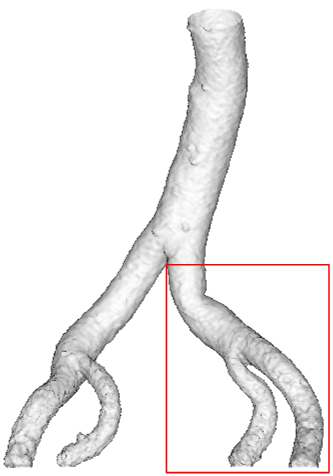
\includegraphics[height=2.4in]{Figures/chap05/VOI.png}
\caption{The original model surface (consists of $205,590$ polygons) and the VOI-extracted local part (in red square).}
\label{fig:VOI}
\end{figure}

%\subsection{Preprocessing for Centerline Extraction}

\subsection{Validating Connectivity of Image-Based Surface Model}

Before actually extracting the centerlines, the image-based surface model of the vasculature needs to be properly conditioned such that the computation can be operated successfully. %
The initial pass is the validation of the connectivity among the adjacent polygonal surfaces that consists of the whole visualization model.
The aim of this step is to find and connect the largest connected region in the given surface model (see Fig. \ref{fig:ConnectivityLocal}).
Table \ref{tbl:Connectivity} shows that the quantities of the consisting polygonal surfaces were not changed in local cases, whilst were decreased in global cases.
The former implies that the given (local) model was the largest connected region in the surface model before the validation.
The latter indicates that the largest connected region of the given model surface was fully extracted through the validation.
\begin{figure}[t]
\centering
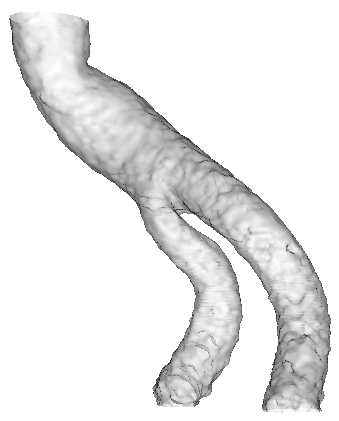
\includegraphics[width=1.5in]{Figures/chap05/connectivity_local.png}
\caption{Results of connectivity validation of model surface in local details (quantity of consisting polygons: $70,625$).}
\label{fig:ConnectivityLocal}
\end{figure}

\begin{table}[t]
\renewcommand{\arraystretch}{1.3}
\caption{Quantities of polygons before and after connectivity validation}
\label{tbl:Connectivity}
\centering
\begin{tabular}
{@{}llr@{}}
%{@{}llrr@{}}
\toprule
%\hline
%~      & ~                       & \multicolumn{2}{c}{Quantities} \\
%\cmidrule(4){3-4}
%~      & ~                       & Vertices & Polygons            \\
~      &                         & Quantities of polygons \\
%\midrule
\hline\hline
%Local  & Before validation       & N/A      & 70,625  \\
%~      & After validation        & N/A      & 70,625  \\
Local  & Before validation       & $70,625$  \\
~      & After validation        & $70,625$  \\
\hline\hline
%Global & Before validation       & N/A      & 205,590 \\
%~      & After validation        & N/A      & 205,452 \\
Global & Before validation       & $205,590$ \\
~      & After validation        & $205,452$ \\
\bottomrule
%\hline
\end{tabular}
\end{table}
\begin{figure}[t]
\centering
\subfloat[]{\includegraphics[width=1.5in]{Figures/chap05/smooth_30_1_local.png}%
\label{fig:Smooth30-1Local}}
\hfil
\subfloat[]{\includegraphics[width=1.45in]{Figures/chap05/smooth_30_01_local.png}%
\label{fig:Smooth30-01Local}}
\hfil
\subfloat[]{\includegraphics[width=1.5in]{Figures/chap05/smooth_100_1_local.png}%
\label{fig:Smooth100-1Local}}
\hfil
\subfloat[]{\includegraphics[width=1.45in]{Figures/chap05/smooth_100_01_local.png}%
\label{fig:Smooth100-01Local}}
\caption{Smoothing effects by applying different parameters: (a) $\text{pass band} = 0.1$, $\text{iterations} = 30$; (b) $\text{pass band} = 0.01$, $\text{iterations} = 30$; (c) $\text{pass band} = 0.1$, $\text{iterations} = 100$; (d) $\text{pass band} = 0.01$, $\text{iterations} = 100$.}%
\label{fig:SmoothLocal}
\end{figure}

%\begin{table}
%\renewcommand{\arraystretch}{1.3}
%\caption{Comparison of quantities of polygonal surfaces - Part I}
%\label{tbl:Eigenvalues}
%\centering
%\begin{tabular}{l||r}
%\hline
%\bfseries Connectivity validation & \bfseries Quantities \\
%\hline\hline
%Before                            & 757,538 \\
%After                             & 757,400 \\
%\hline
%\end{tabular}
%\end{table}

\subsection{Smoothing Connected Surface Model}

The centerline extracting method adopted in this work is sensitive to the noises on the input surface.
Due to the poor quality in some level of details of the original images, segmentation may introduce unnecessary uneven surfaces.
These artifacts in the surfaces can cause difficulties in the delivering of the virtual guidewires towards the hesion along the lumen of the model vessels.
To depress the noisy surface of the model, a surface smoothing module implemented based on low-pass filtering is applied.
There are two parameters associated with the smoothing module.
One of them specifies the number of iterations, which is equivalent to the degree of the polynomial approximating the windowed sinc function defined by (\ref{eqn:Approximation}).
The other determines the pass band of this low-pass filtering module.
Different sets of parameters were fed to the smoothing module in order to find the best results for the following processing (see Fig. \ref{fig:SmoothLocal}).
Observing these results, the parameters ($\text{pass band} = 0.01$, $\text{iterations} = 100$) used to generating the resulting surface in Fig. \ref{fig:Smooth100-01Local} demonstrated better effects than the rest.
%\begin{figure}[t]
%\centering
%\subfloat[]{\includegraphics[width=1.5in]{../Figures/smooth_30_1_local.eps}%
%\label{fig:Smooth30-1Local}}
%\hfil
%\subfloat[]{\includegraphics[width=1.45in]{../Figures/smooth_30_01_local.eps}%
%\label{fig:Smooth30-01Local}}
%\hfil
%\subfloat[]{\includegraphics[width=1.5in]{../Figures/smooth_100_1_local.eps}%
%\label{fig:Smooth100-1Local}}
%\hfil
%\subfloat[]{\includegraphics[width=1.45in]{../Figures/smooth_100_01_local.eps}%
%\label{fig:Smooth100-01Local}}
%\caption{Smoothing effects by applying different parameters: (a) $\text{pass band} = 0.1$, $\text{iterations} = 30$; (b) $\text{pass band} = 0.01$, $\text{iterations} = 30$; (c) $\text{pass band} = 0.1$, $\text{iterations} = 100$; (d) $\text{pass band} = 0.01$, $\text{iterations} = 100$.}%
%\label{fig:SmoothLocal}
%\end{figure}

\subsection{Subdivision Using Improved Butterfly Scheme}

To further attenuate the effects of noisy surfaces on extraction of centerlines and increase the precision of the centerlines extraction, the number of the polygons consisting the model surface has to be increased.
In order to achieve this, the smoothed surface need to be subdivided without introducing more perturbation.
Figure \ref{fig:SubdivisionLocal} illustrates that the subdivision computation based on the improved butterfly scheme.
At the same time, the quantities of the consisting polygonal surfaces increased substantially after the subdivision complete (see Table \ref{tbl:Subdivision}).
Comparing the quantities of the polygons before and after the subdivision in both cases, the quantities of the resulting polygons are about four times greater than the quantities of the input polygons due to the subdivision scheme employed in this work.
\begin{figure}[t]
\centering
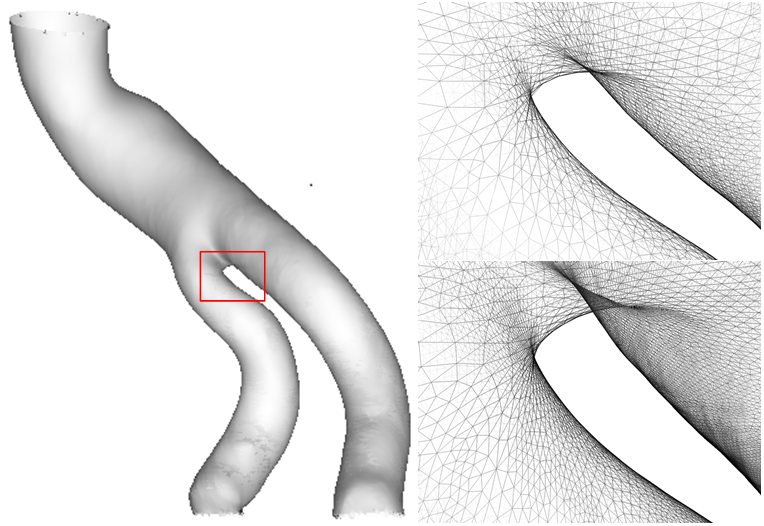
\includegraphics[width=3.0in]{Figures/chap05/subdivision.png}
\caption{Subdivision of smoothed surface by using improved butterfly scheme. \emph{Left}: subdivision in local details. \emph{Top right}: polyhedral surface before subdivision. \emph{Bottom right}: polyhedral surface after subdivision.}%
\label{fig:SubdivisionLocal}
\end{figure}

\begin{table}[t]
\renewcommand{\arraystretch}{1.3}
\caption{Quantities of polygons before and after subdivision using an improved butterfly scheme}
\label{tbl:Subdivision}
\centering
\begin{tabular}
%{@{}llr@{}}
{@{}llrr@{}}
\toprule
%\hline
%~      & ~                       & \multicolumn{2}{c}{Quantities} \\
%\cmidrule(4){3-4}
%~      & ~                       & Vertices & Polygons            \\
~      &                         & Quantities of polygons & Percentages ($\%$)\\
%\midrule
\hline\hline
%Local  & Before subdivision      & N/A      &  70,625  \\
%~      & After subdivision       & N/A      & 281,060  \\
Local  & Before subdivision      &  $70,625$  &\\
~      & After subdivision       & $281,060$  & 398 \\
\hline\hline
%Global & Before validation       & N/A      & 205,452  \\
%~      & After validation        & N/A      & 821,808  \\
Global & Before validation       & $205,452$  &\\
~      & After validation        & $821,808$  & 400 \\
\bottomrule
%\hline
\end{tabular}
\end{table}

%\begin{table}
%\renewcommand{\arraystretch}{1.3}
%\caption{Comparison of quantities of polygonal surfaces - Part II}
%\label{tbl:Eigenvalues}
%\centering
%\begin{tabular}{l||r}
%\hline
%\bfseries Subdivision  & \bfseries Quantities \\
%\hline\hline
%Before                 &  757,400 \\
%After                  & 3,029,600 \\
%\hline
%\end{tabular}
%\end{table}

\begin{figure}[t]
\centering
\subfloat[]{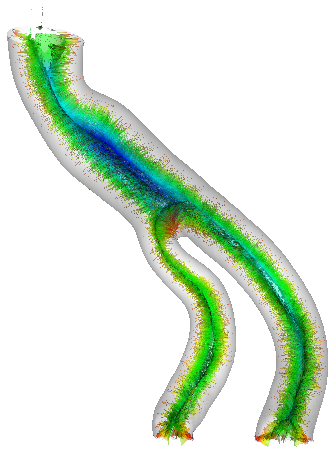
\includegraphics[width=1.5in]{Figures/chap05/overlay_100_01_voronoi_local.png}%
\label{fig:VoronoiLocal}}
\hfil
\subfloat[]{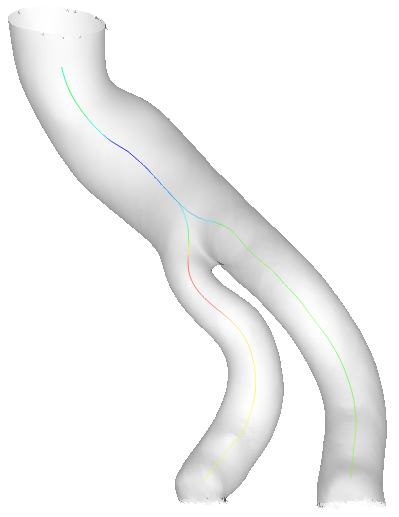
\includegraphics[width=1.5in]{Figures/chap05/overlay_100_01_centerlines_local.png}%
\label{fig:OverlayLocal}}
\caption{Centerlines extraction of the aorta in local details: (a) embedded Voronoi diagram; (b) centerlines inside the vessel.}%
\label{fig:CenterlinesLocal}
\end{figure}

\begin{figure}[t]
\centering
\subfloat[]{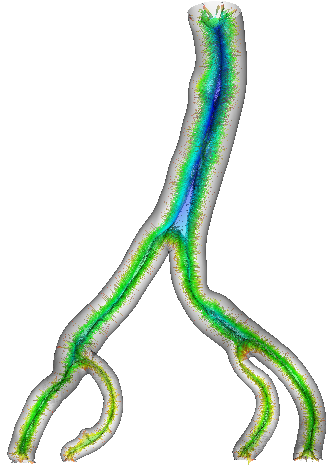
\includegraphics[height=2.0in]{Figures/chap05/overlay_100_01_voronoi.png}
%\caption{Voronoi diagrams of the abdominal aorta.}
\label{fig:VoronoiGlobal}}
\hfil
\subfloat[]{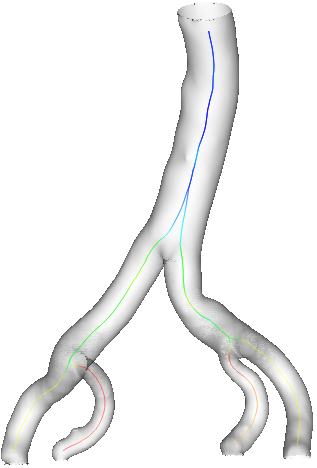
\includegraphics[height=2.0in]{Figures/chap05/overlay_100_01_centerlines.png}
%\caption{Centerlines of the abdominal aorta.}
\label{fig:OverlayGlobal}}
\caption{Centerlines extraction of the aorta in VOI. (a) Voronoi diagrams; (b) Centerlines. }
\label{fig:CenterlineGlobal}
\end{figure}

\subsection{Centerlines Extraction Based on Surface Model}

The centerlines extraction computation was performed on the subdivided surface model.
Firstly, the embedded Voronoi diagram of the preprocessed surface model is generated (see Fig. \ref{fig:VoronoiLocal}).
Secondly, the centerlines of the tubular surface model is computed (see Fig. \ref{fig:OverlayLocal}).
The colors marked on the Voronoi diagram and the centerlines denote the diameters of the local resection circle, decreasing from blue to red.
The same processing was straightly applied to the model surface of the whole abdominal aorta (see Fig. \ref{fig:VoronoiGlobal} and Fig. \ref{fig:OverlayGlobal}).
One can see from the details of the results that the starting and ending points are not exactly located at the ``entrances" or ``exits".
The reason of this is the Voronoi diagram on which the points consisting the centerlines exist never intersect with the model surface, i.e., the ending points of the centerlines are approaching the terminals of the surface model as near as possible, but never stick to them.
\begin{figure}[t]
\centering
\subfloat[]{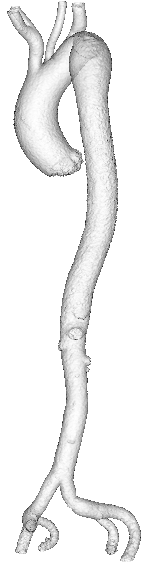
\includegraphics[width=0.7in]{Figures/chap05/surface.png}%
\label{fig:SurfaceModel}}
\hfil
\subfloat[]{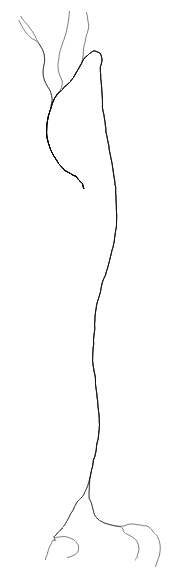
\includegraphics[width=0.9in]{Figures/chap05/centerlines.png}%
\label{fig:CenterlinesModel}}
\caption{Visualization models of the aorta: (a) image-based surface model (quantity of consisting polygons: $757,538$); (b) centerlines of the surface model.}%
\label{fig:VisualizationModel}
\end{figure}

\subsection{Discussions}

The computer programs used in this paper were written in C++ based on the Visualization Toolkit, an open source library aims at providing general facilities in the scientific visualization field \cite{Schroeder2000VTK}. %
To depress the unintended affections of the unstructured polygonal surfaces and the noises introduced by the image segmentation, series of steps were introduced in our experiments to extract the centerlines of the surface model of the vasculature. %
During this process, the quantities of the consisting polygons were obviously decreased for the extraction of the largest connected region in the surface model.
Due to the centerlines extraction computation is sensitive and expensive, we subdivided the smoothed surface model based on an improved butterfly scheme.
After this process, the quantities of the consisting polygonal surfaces were increased because of the refinement of the polygons.
With this step, the potential perturbation was further reduced, leading to much less errors which may occur during the computation of the centerlines extraction.
It is noteworthy that the extraction of centerlines for the model surface is an expensive computation both in time and space.
The calculation of the whole aorta (see Fig. \ref{fig:VisualizationModel}) cost nearly eight hours on our desktop machine with dedicated modification on the code to fit the bulky data into the relatively limited memory. %
%The calculation of the whole aorta cost nearly eight hours on our desktop machine with dedicated modification on the code to fit the bulky data into the relatively limited memory. %
